\documentclass[11pt]{article}
\usepackage{graphicx}
\graphicspath{ {images/} }
\usepackage[rightcaption]{sidecap}
\usepackage{svg}
\usepackage{transparent}
\usepackage{xcolor}
\usepackage{relsize}
\usepackage{amsmath}
\usepackage{amsfonts}
\usepackage[margin=2cm]{geometry}
\usepackage{fancyhdr}
\usepackage{enumitem}
\usepackage{natbib}
\pagestyle{fancy}
\usepackage{float}
\usepackage[utf8]{inputenc}
\numberwithin{equation}{subsection}

\title{Approximation of Experimental Physical Values with Non-typical Conditions of Error}
\date{\today}

\DeclareRobustCommand\dash{%
  \unskip\nobreak\thinspace\textemdash\allowbreak\thinspace\ignorespaces}

\DeclareUnicodeCharacter{0177}{\^y}
\begin{document}
%TITLE
\begin{titlepage}
\begin{center}
\pagenumbering{0}
IB Mathematics Higher Level Internal Assessment on Statistics 
\\ 
\rule{\textwidth}{0.25pt}
\linebreak
\Huge{Approximation of Experimental Physical Values with Non-typical Conditions of Error}
\rule{\textwidth}{0.25pt} \\
[15cm]
\large {David Simon Tetruashvili} \\

\end{center}
\end{titlepage}
\newpage
%TITLE END

%TOC
\tableofcontents
\pagenumbering{arabic}
\newpage
%TOC END

%Body
\section{Introduction}

\section{Mathematical Background}

\section{Formulation of the Problem}

A function is one of the most known mathematical objects. An important task which has practical applications, is the approximation of a function or relationship based on some information known about the function or relationship in question. This information may either be determinate or statistical. An example of a determinate piece of information about function $f(x)$ is its range (or the possible values this function may have) on a given interval $[\alpha,\beta]$. Example of a statistical information may be the law of distribution of random errors $\xi_{i}$ in approximate values $\tilde{y}_{i} = f(x_{i})+\xi_{i}$ of the function, which in turn can describe a certain physical process (change of temperature over time, for example). In practice, a number $n$ of points $x_{i}$ can be obtained as results of some kind of physical experiment. Where in this case, the approximation of function $f(x)$ only makes sense if the this function is described by a finite number $m<n$ of parameters (coefficients) $c_{j}$, where the true values of said parameters will be denoted as $\dot{c}_{j}, \ j=1,2,\dots,m.$ \\
\\
This Internal Assessment will focus on the estimation of parameters of the function
\begin{equation}
y = f(\dot{c},x_{i}),\quad \dot{c} \in \boldsymbol{R}^{m},\quad x \in [\alpha,\beta],\quad \dot{c} = (\dot{c}_{1}, \dot{c}_{2},\dots,\dot{c}_{m}) \label{301}
\end{equation}
based on its approximate values
\begin{equation}
\tilde{y}_{i} = f(x_{i})+\xi_{i}, \quad i=1,2,\dots,n ,
\end{equation}
when additionally it is also known, that: 1. vector $\dot{c} = (\dot{c}_{1}, \dot{c}_{2},\dots,\dot{c}_{m})$ belongs to a given limited set $D$, like for example a parallelepiped in $\boldsymbol{R}^{m}$ dimensions; 2. $\xi$ is a limited continuous random value; the median of which $Med(\xi)$ is equal to zero. \\
\\
Judging by references in scientific works that I read while researching for this IA [*], the most popular linear model of a studied relationship is
\begin{equation}
f(\dot{c},x)= \sum\limits_{j=1}^{m} \dot{c}_{j} \phi_{j}(x),
\end{equation}
specifically in polynomial form, when
\begin{equation}
\phi_{1}(x)\equiv 1; \quad \phi_{j}(x)=x^{j-1},\quad j=1,2,\dots,m.
\end{equation}
\\
In practice, it is often the case when it is not only necessary to estimate the parameters of a function, but identifying the type (structure) of this function is needed as well. In other words, a finite number $L$ of alternative structures is given
\begin{equation}
f_{l}(c;x), c \in \boldsymbol{R}^{m(l)}, \quad l=1,2,\dots,L,
\end{equation}
and it is necessary to identify to which of $L$ structures of function $f_{l}(c;x)$ belongs the function $f(\dot{c},x)$, and after that estimate the vector $\dot{c}$ of its parameters. In our school program, the class has encountered one such task, when it was said to find out if we were dealing with a linear or exponential relationship, be it in either physics or math. However, then, this problem was solved using the exact (or near to exact) values of both of the relationships, so it was easy to distinguish them. \\
\\
There are countless papers dedicated to the approximation of functions based on their approximate values (in practice - experimental data). Usually, in such papers the consensus is to use a certain condition. This condition is to assume that the mathematical expectancy of error is equal to zero [*].
\begin{equation}
E(\xi)=0
\end{equation}
 However, in this IA this condition will not be used. Here instead of the condition of mathematical expectancy of error $\xi$ being equal to zero, I will assume that the median of the same error $\xi$ being equal to zero, 
\begin{equation}
Med(\xi)=0
\end{equation}
specifically when the algorithm of evaluation of the parameters of the function is based on ideas from the \textit{method of least squares}. \\
\\
I justify my interest to the condition $Med(\xi)=0$ by the case when the traditional condition $E(\xi)=0$ is unachievable. This happens when measurements are taken close to one of the natural limits of the physical relationship being measured. An example of such natural limit is the inability of some magnitude, such as weight, to be negative. In this case, the absolute value of the error made, can only be large (with respect to other errors made) in the \textit{same sign}, either positive or negative. Figure \ref{fig:graph-nl} shows an example of this graphically.
\begin{figure}[h!]
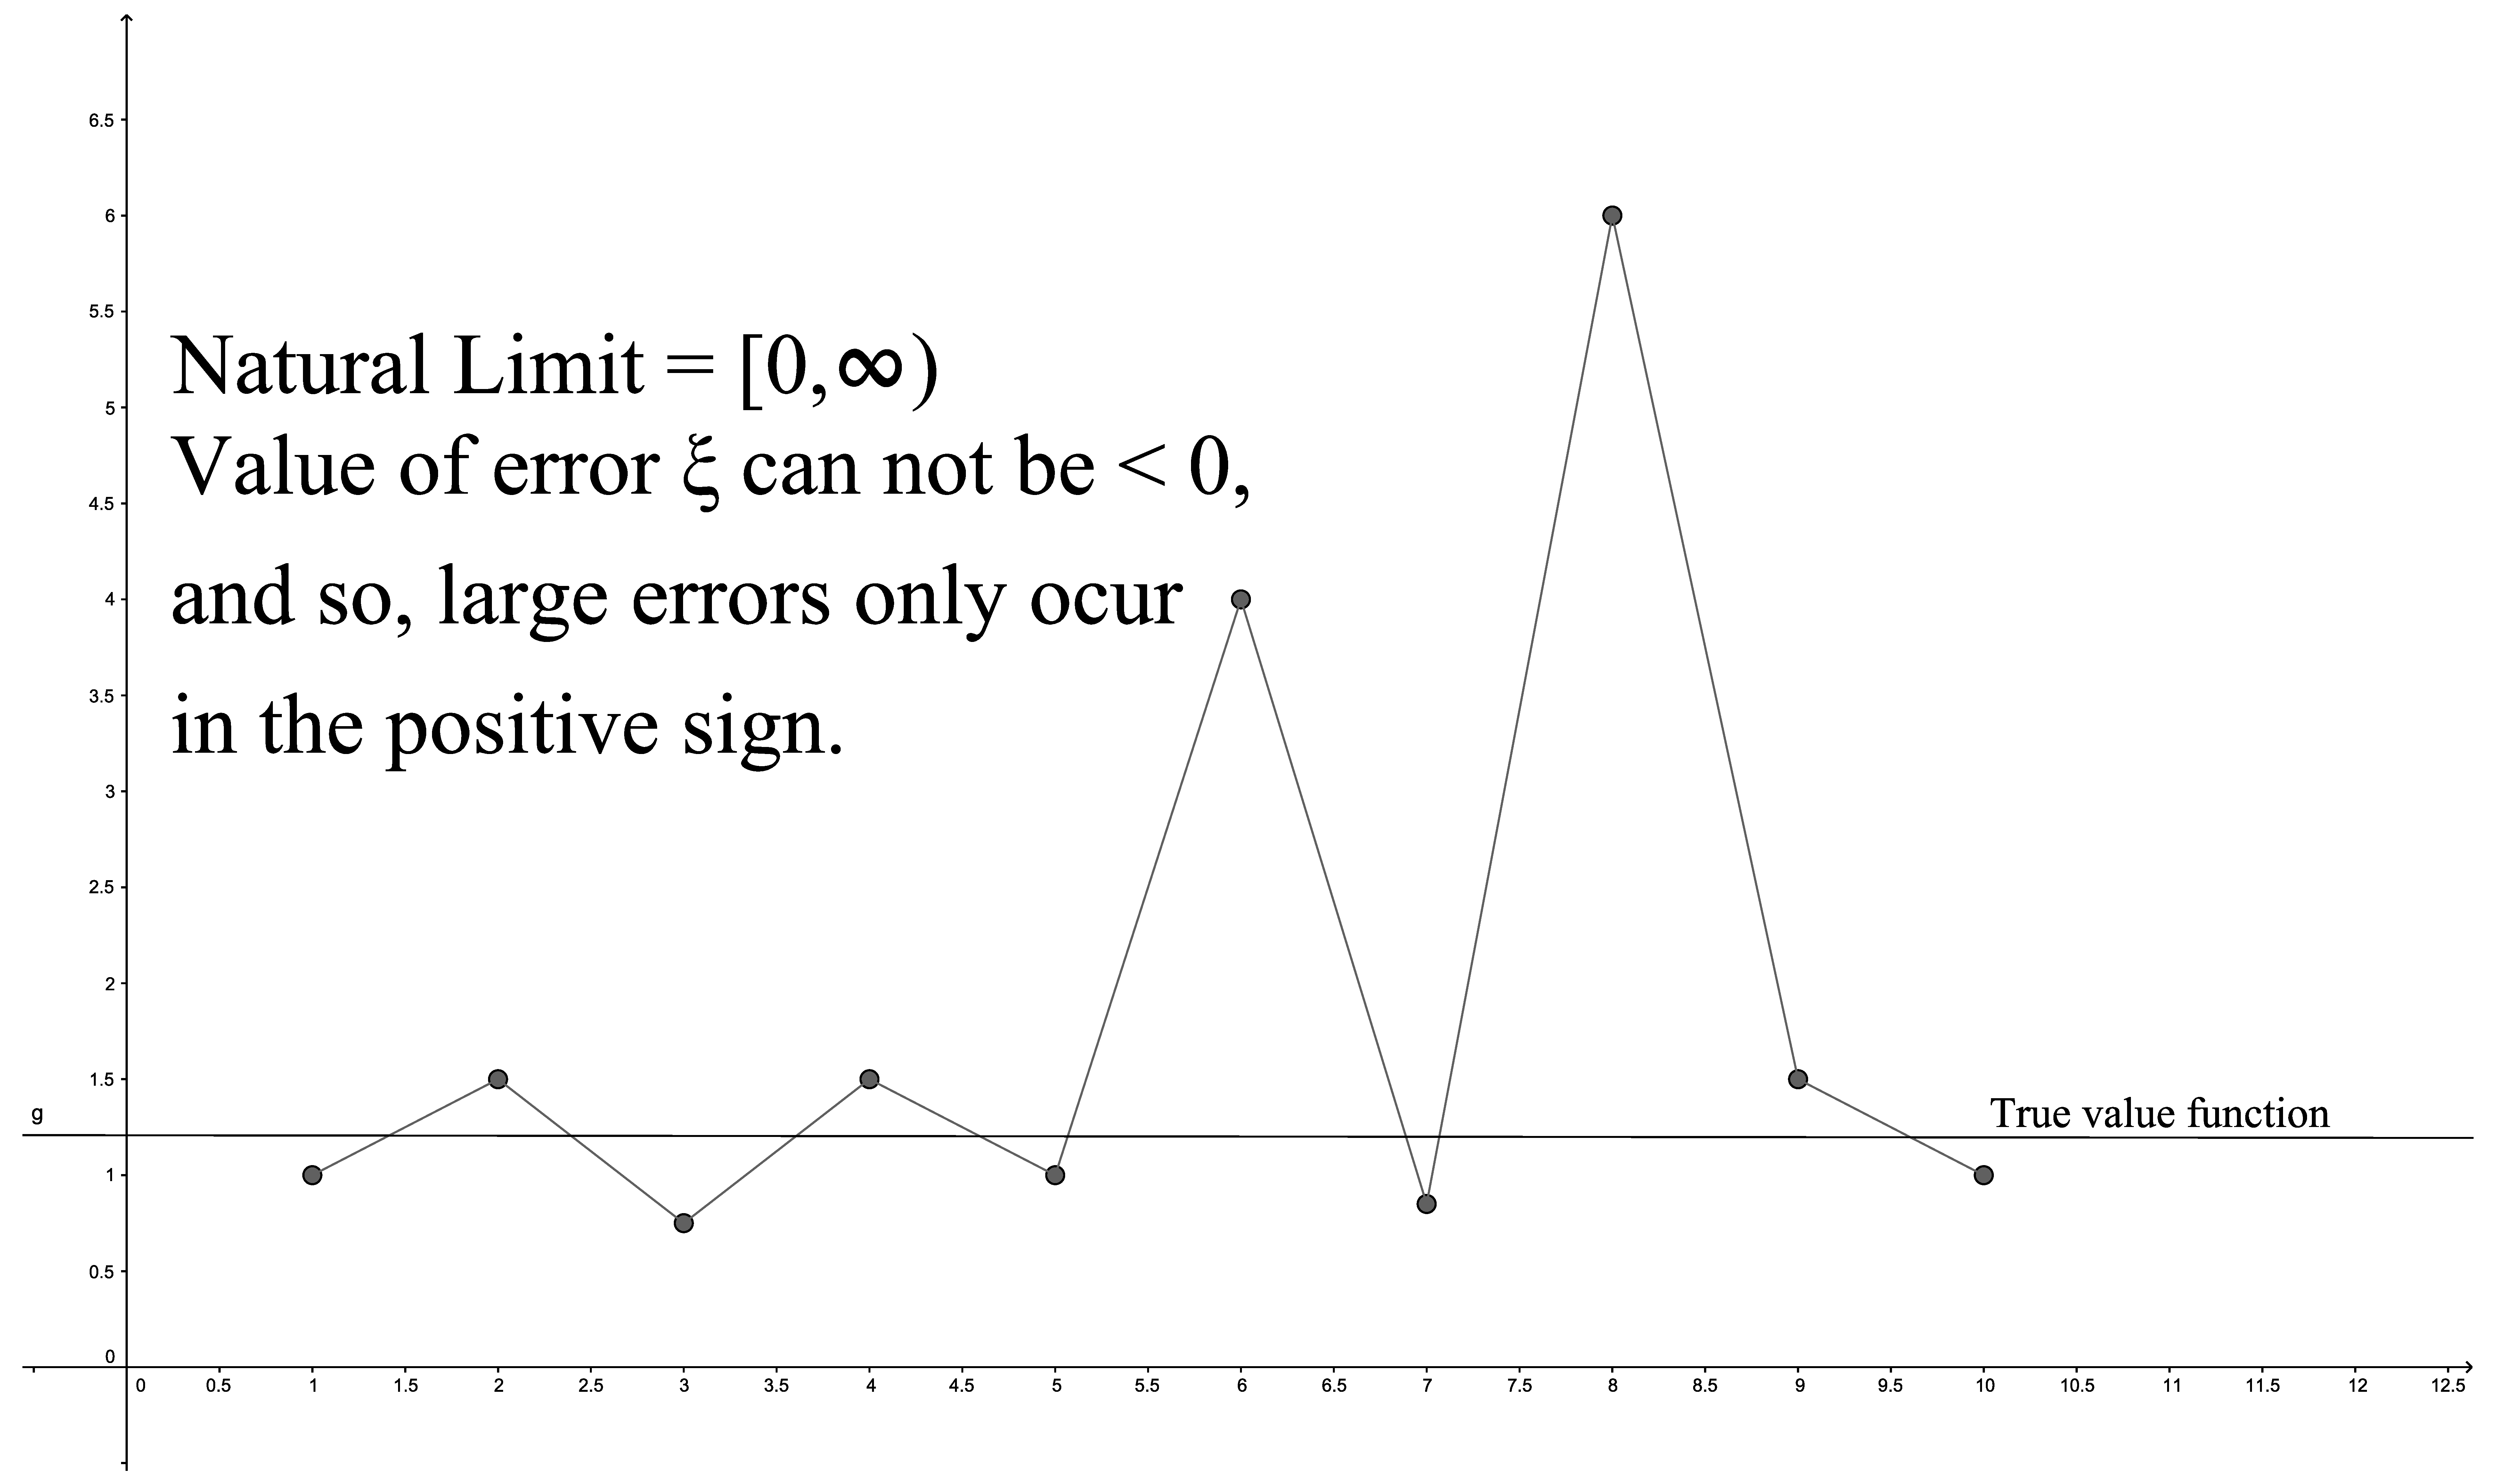
\includegraphics[scale=0.07]{natural_limits}
\centering
\caption{Graphical representation of a case where $E(\xi)=0$ does not work effectively.}
\label{fig:graph-nl}
\end{figure}
\\
Speaking of the errors, what is meant is not only error that was produced by a faulty measurement, but also any error caused by some factor that was either omitted or unaccounted for in function $f(x)$. Even though both conditions $E(\xi)=0$ and $Med(\xi)=0$ are not special cases of each other,it could be argued that from a point of view of solving practical problems, the condition $Med(\xi)=0$ is the more broad of the two (as in, it is easier to meet). The only requirement for meeting this condition is $P(\xi)>0$ is 0.5.  Hence the condition $Med(\xi)=0$ allows for some comparatively large random values of error $\xi$ to be on one side of the true function and not on the other, without the approximation to be significantly affected by those large values, unlike the condition $E(\xi)=0$. With condition $Med(\xi)=0$ the approximation can account for large peaks in values of $\xi$.\\
\\
As mentioned before, I have two aims in this IA. Aim-maximum - to create an algorithm, capable of identifying from a finite number of alternative function structures, to which of those does the relationship in question belong; estimate the parameters of this function accurately; quite securely give an estimate to the accuracy of the calculated approximate values of the function, which belong to the relationship in question. Aim-minimum - to create an algorithm, capable of estimating the parameters of a functional dependence whose structure is known accurately; again, securely give an estimate to the accuracy of the calculated approximate values of the functional dependence. \\
\\
Its clear that the quality of the solution of this problem is dependant of an array of factors, which include: 1. the ratio between the number $n$ of measurements $\tilde{y}_{i}$ and the number $m$ of estimated parameters $\dot{c}_{j}$. 2. the intensity of error $\xi_{i}$ 3. the number of $L$ alternatives, and more importantly, the degree of similarity of functions $f_{l}(c;x)$. This means that to confirm my theoretical reasoning, quite an ambitions computational experiment is required. I will proceed with the necessary calculations using custom software. 

\section{Algorithm}



\section{Given Examples}

\section{Conclusion and Reflection}
\newpage

\section*{Biblyography}
\end{document}

